\documentclass[aspectratio=169]{beamer}

\usepackage{amssymb,amsmath}
\usepackage{graphicx}
\usepackage{url}
\usepackage{color}
\usepackage{pagenote}[continuous,page]
\usepackage{relsize}		% For \smaller
\usepackage{url}			% For \url
\usepackage{epstopdf}	% Included EPS files automatically converted to PDF to include with pdflatex

%For MindMaps
% \usepackage{tikz}%
% \usetikzlibrary{mindmap,trees,arrows}%

%%% Color Definitions %%%%%%%%%%%%%%%%%%%%%%%%%%%%%%%%%%%%%%%%%%%%%%%%%%%%%%%%%
%\definecolor{bordercol}{RGB}{40,40,40}
%\definecolor{headercol1}{RGB}{186,215,230}
%\definecolor{headercol2}{RGB}{80,80,80}
%\definecolor{headerfontcol}{RGB}{0,0,0}
%\definecolor{boxcolor}{RGB}{186,215,230}

%%% Save space in lists. Use this after the opening of the list %%%%%%%%%%%%%%%%
%\newcommand{\compresslist}{
%	\setlength{\itemsep}{1pt}
%	\setlength{\parskip}{0pt}
%	\setlength{\parsep}{0pt}
%}

%\setbeameroption{show notes on top}

% You should run 'pdflatex' TWICE, because of TOC issues.

% Rename this file.  A common temptation for first-time slide makers
% is to name it something like ``my_talk.tex'' or
% ``john_doe_talk.tex'' or even ``discrete_math_seminar_talk.tex''.
% You really won't like any of these titles the second time you give a
% talk.  Try naming your tex file something more descriptive, like
% ``riemann_hypothesis_short_proof_talk.tex''.  Even better (in case
% you recycle 99% of a talk, but still want to change a little, and
% retain copies of each), how about
% ``riemann_hypothesis_short_proof_MIT-Colloquium.2000-01-01.tex''?

\mode<presentation>
{
  \usetheme{CambridgeUS}		% bem bacana - menu superior
  \usecolortheme{default}		% branco, azul clarinho
  \useoutertheme{default}
  \useinnertheme{circles}
  \setbeamercovered{invisible}
}

\beamertemplatenavigationsymbolsempty

%% Better looking blocks
\setbeamercolor{block title alerted}{use=structure,fg=black,bg=red!80!black}
\setbeamercolor{block body alerted}{use=structure,fg=black,bg=white!90!black}

\setbeamercolor{block title}{use=structure,fg=black,bg=blue!60!white}
\setbeamercolor{block body}{use=structure,fg=black,bg=white!90!black}

\usepackage[english]{babel}
\usepackage[latin1]{inputenc}
\usepackage{subfigure}

\usepackage{times}
\usepackage[T1]{fontenc}

%% makes the ppagenote command for figure references at the end.
\makepagenote
\renewcommand{\notenumintext}[1]{}
\newcommand{\ppagenote}[1]{\pagenote[Page \insertframenumber]{#1}}


\usepackage{tikz}
\usetikzlibrary{arrows,shapes}

\title[GB13604]{GB13604 - Maths for Computer Science}
\subtitle[]{Lecture 4 -- Graphs Part I}
\author[Claus Aranha]{Claus Aranha\\{\footnotesize caranha@cs.tsukuba.ac.jp}}
\institute[COINS]{College of Information Science}
\date[2018-10-28]{2018-10-28\\{\tiny Last updated \today}}

\tikzstyle{vertex}=[circle,fill=black!25,minimum size=10pt,inner sep=0pt]
\tikzstyle{blue vertex}=[circle,fill=blue!100,minimum size=10pt,inner sep=0pt]
\tikzstyle{red vertex}=[circle,fill=red!100,minimum size=10pt,inner sep=0pt]
\tikzstyle{edge} = [draw,thick,-]
\tikzstyle{pedge} = [draw,thick,.]
\tikzstyle{red edge} = [draw, thick,-,red!50]
\tikzstyle{black edge} = [draw, line width=2pt,-,black!20]
\tikzstyle{weight} = [font=\smaller]

\begin{document}

\begin{frame}
  \maketitle

  \begin{columns}
    \column{0.8\textwidth}
    {\smaller This course is based on Mathematics for Computer Science, Spring
    2015, by Albert Meyer and Adam Chlipala, Massachusetts Institute
    of Technology OpenCourseWare.}
    \column{0.2\textwidth}
    
\includegraphics[width=\textwidth]{../img/by-nc-sa}
  \end{columns}
\end{frame}

\begin{frame}{Graphs -- Lectures 4 and 5}
  \begin{columns}
    \column{0.5\textwidth}
    \begin{center}
      Lecture I: Chapter 9
    \end{center}
    \begin{itemize}
      \item Graphs and Relations
      \item Directed Graphs and Walks
      \item Scheduling and Partial Orders
    \end{itemize}

    \column{0.5\textwidth}
    \begin{center}
      Lecture II: Chapter 11
    \end{center}
    \begin{itemize}
    \item Using Isomorphism
    \item Coloring and Connectivity
    \item Spanning Trees
    \item Matching
    \end{itemize}
  \end{columns}
\end{frame}

% Graphs
% Walks
% Partial Orders
% Isomorphism

\section{Graphs}

\frame{
{Part 1: Graph Definitions}

\tableofcontents[currentsection,hideallsubsections, firstsection=1, sections={1-3}]
}

\subsection{Motivations}

\begin{frame}{Using Graphs to Solve Problems}{Course Registration}

  We can represent a list of courses in a university, and their requirements, using a graph structure. For example, to take \emph{"Computer Graphics"}, you need to take \emph{"Programming Theory"} and \emph{"Linear Algebra"} first.\medskip

  If you take two lectures per semester, how long would it take you to graduate? Why?

  \begin{tabular}{p{.1\textwidth}|p{.45\textwidth}||p{.3\textwidth}}
    \hline
    Code & Lecture & Prerequisites \\
    \hline
    0000 & {\small Social Questions} & \emph{none} \\
    0001 & {\small Intro to Programming} & \emph{none} \\
    0002 & {\small Calculus I} & \emph{none} \\
    0003 & {\small Programming Theory} & \emph{0001} \\
    0004 & {\small Linear Algebra} & \emph{0000, 0002} \\
    0005 & {\small Programming Challenges} & \emph{0000, 0001, 0003} \\
    0006 & {\small Computer Graphics} & \emph{0003, 0004} \\
    \hline
  \end{tabular}
\end{frame}


\begin{frame}{Using Graphs to Solve Problems}{Course Registration}

  The university proposes a new lecture, \emph{"Maths for Computer Science"}. The updated table is below. \medskip

  How long does it take to graduate now? Why?

  \begin{tabular}{p{.1\textwidth}|p{.45\textwidth}||p{.3\textwidth}}
    \hline
    Code & Lecture & Prerequisites \\
    \hline
    0000 & {\small Social Questions} & \emph{none} \\
    0001 & {\small Intro to Programming} & \emph{none} \\
    0002 & {\small Calculus I} & \emph{none} \\
    0003 & {\small Programming Theory} & \emph{0001, {\bf 0007}} \\
    0004 & {\small Linear Algebra} & \emph{0000, 0002} \\
    0005 & {\small Programming Challenges} & \emph{0000, 0001, 0003} \\
    0006 & {\small Computer Graphics} & \emph{0003, 0004} \\
    {\bf 0007} & {\small {\bf Maths for Computer Science}} & {\bf\emph{0005}} \\
    \hline
  \end{tabular}
\end{frame}

\begin{frame}{Using Graphs to Solve Problems}{Airplane}
  \begin{columns}

    \column{0.3\textwidth}
    In an airport, each airplane needs a gate when it is on the ground.\medskip

    If we know the landing and departing time of each plane, what is the minimum number of gates necessary?
    \column{0.7\textwidth}
    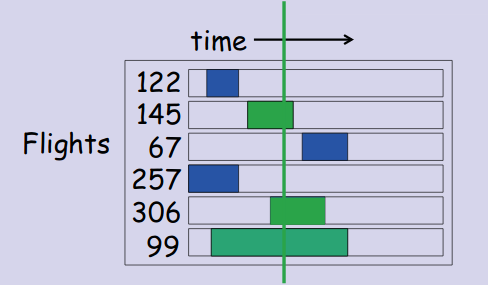
\includegraphics[width=\textwidth]{../img/gatetable}
  \end{columns}
\end{frame}

\begin{frame}[t]{Problems as Graphs}
  Many problems that can be described by the \emph{relationship} betwene entities in the problem can be represented as graphs.\bigskip

  \begin{itemize}
    \item A course is a prerequisite to another one;
    \item Two planes are landed at the same time;
    \item Webpages and the links between them;
  \end{itemize}\bigskip

  These relationships can be described mathematically using a graph structure.
\end{frame}

\subsection{Definitions}

\begin{frame}[t]{Graph Basic Definitions}

    \begin{columns}
      \column{0.4\textwidth}
      \begin{center}
        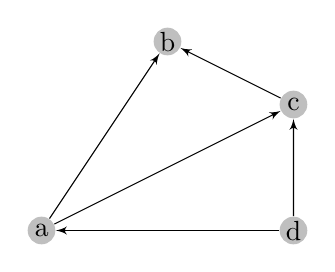
\begin{tikzpicture}[scale=.8,auto,swap]
  \tikzset{edge/.style = {->,>=latex'}}
  \node[vertex] (a) at (0,0) {a};
  \node[vertex] (b) at (2,3) {b};
  \node[vertex] (c) at (4,2) {c};
    \node[vertex] (d) at (4,0) {d};
    \draw[edge] (a) to (b);
    \draw[edge] (a) to (c);
    \draw[edge] (c) to (b);
    \draw[edge] (d) to (c);
    \draw[edge] (d) to (a);
\end{tikzpicture}

      \end{center}

      \column{0.6\textwidth}
        A {\bf graph} $G$ is defined by a set of vertices $V$, and a set of edges $E$.\bigskip

        \begin{itemize}
          \item $G = (V,E)$
          \item $V = \{a,b,c,d\}$
          \item $E = \{(a,b), (a,c), (c,b), (d,c), (d,a)\}$
        \end{itemize}\bigskip

         A {\bf directed graph (digraph)} is a graph where each edge has a {\bf direction}.\medskip

         An {\bf undirected graph} is a graph where the edges do not have a direction ($(a,b) \iff (b,a)$).
    \end{columns}
\end{frame}

\begin{frame}{Graphs and Relations}{Remember Lecture 2?}

  \begin{columns}
    \column{0.4\textwidth}
    \begin{center}
      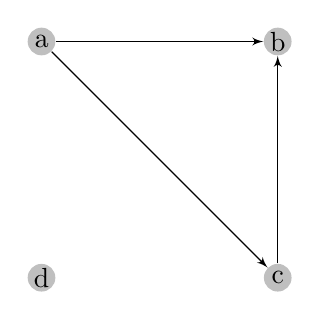
\begin{tikzpicture}[scale=3,auto,swap]
      \tikzset{edge/.style = {->,>=latex'}}
      \node[vertex] (a) at (0,1) {a};
      \node[vertex] (b) at (1,1) {b};
      \node[vertex] (c) at (1,0) {c};
      \node[vertex] (d) at (0,0) {d};
      \draw[edge] (a) to (c);
      \draw[edge] (a) to (b);
      \draw[edge] (c) to (b);
      \end{tikzpicture}
    \end{center}
    \column{0.6\textwidth}

    Graph $G = (V, E)$
    \begin{itemize}
      \item $V = \{a,b,c,d\}$
      \item $E = \{(a,c),(a,b),(c,b)\}$
    \end{itemize}\bigskip

    A digraph with vertices $V$ can be understood as a \structure{binary relation $V \to V$}\bigskip

    In the same way, every \structure{binary relation} can be written as a directed graph too.
  \end{columns}
\end{frame}

\begin{frame}{Matrix Representation of a Digraph}

  \begin{columns}
    \column{0.5\textwidth}
    \begin{center}
    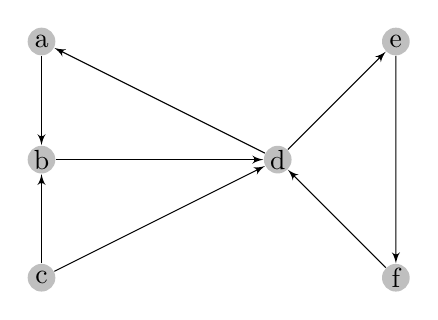
\begin{tikzpicture}[scale=1.5,auto,swap]
      \tikzset{edge/.style = {->,>=latex'}}
      \node[vertex] (a) at (0,1) {a};
      \node[vertex] (b) at (0,0) {b};
      \node[vertex] (c) at (0,-1) {c};
      \node[vertex] (d) at (2,0) {d};
      \node[vertex] (e) at (3,1) {e};
      \node[vertex] (f) at (3,-1) {f};
      \draw[edge] (a) to (b);
      \draw[edge] (c) to (b);
      \draw[edge] (b) to (d);
      \draw[edge] (d) to (a);
      \draw[edge] (c) to (d);
      \draw[edge] (d) to (e);
      \draw[edge] (e) to (f);
      \draw[edge] (f) to (d);
    \end{tikzpicture}
  \end{center}

    \column{0.5\textwidth}

    {\larger
      \begin{tabular}{c|cccccc}
        & a & b & c & d & e & f \\
        \hline
        a &0&1&0&0&0&0\\
        b &0&0&0&1&0&0\\
        c &0&1&0&1&0&0\\
        d &1&0&0&0&1&0\\
        e &0&0&0&0&0&1\\
        f &0&0&0&1&0&0\\
      \end{tabular}
    }\medskip

    {\bf Adjacency Matrix}
  \end{columns}
  \bigskip

  An \structure{Adjacency Matrix} A represents a digraph, when $A_{i,j}$ is 1 if $v_i \to v_j$, and 0 if not.

  \begin{equation*}
    A(v_i,v_j) = 1 \iff E(v_i) = v_j
  \end{equation*}
\end{frame}

\section{Walks}

\frame{
{Part 2: Walks in Graphs}

\tableofcontents[currentsection,hideallsubsections, firstsection=1, sections={1-3}]
}

\subsection{Walks, Paths and Relations}

\begin{frame}[t]{A solution to a problem can be a set of edges and vertices}

{\bf Question:} Is it possible to graduate in the curriculum below?
\begin{tabular}{p{.1\textwidth}|p{.45\textwidth}||p{.3\textwidth}}
  \hline
  Code & Lecture & Prerequisites \\
  \hline
  0000 & {\small Social Questions} & \emph{none} \\
  0001 & {\small Intro to Programming} & \emph{none} \\
  0002 & {\small Calculus I} & \emph{none} \\
  0003 & {\small Programming Theory} & \emph{0001} \\
  0004 & {\small Linear Algebra} & \emph{0000, 0002} \\
  0005 & {\small Programming Challenges} & \emph{0000, 0001, 0003} \\
  0006 & {\small Computer Graphics} & \emph{0003, 0004} \\
  \hline
\end{tabular}\bigskip 

{\bf Answer:} Create the \emph{curriculum's graph} and find a way to go to all vertices from the starting ones.


\end{frame}


\begin{frame}[t]{Walks and Paths}

  The solution of many graph problems is represented as a sequence of vertices and edges.\bigskip 

  A sequence of vertices in a graph is a \structure{Walk} or a \structure{Path}.\bigskip

  \begin{itemize}
    \item {\bf Walk:} Any sequence of successive edges. 

    \item {\bf Path:} A walk that never visits the same vertex more than once.
  \end{itemize}
\end{frame}

\begin{frame}{Walk example}

  \begin{center}
    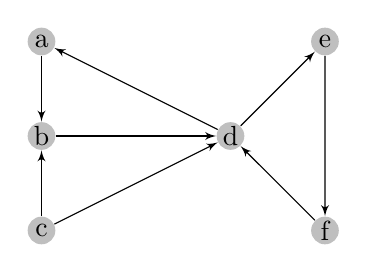
\begin{tikzpicture}[scale=1.2,auto,swap]
      \tikzset{edge/.style = {->,>=latex'}}
      \node[vertex] (a) at (0,1) {a};
      \node[vertex] (b) at (0,0) {b};
      \node[vertex] (c) at (0,-1) {c};
      \node[vertex] (d) at (2,0) {d};
      \node[vertex] (e) at (3,1) {e};
      \node[vertex] (f) at (3,-1) {f};
      \draw[edge] (a) to (b);
      \draw[edge] (c) to (b);
      \draw[edge] (b) to (d);
      \draw[edge] (d) to (a);
      \draw[edge] (c) to (d);
      \draw[edge] (d) to (e);
      \draw[edge] (e) to (f);
      \draw[edge] (f) to (d);
  \end{tikzpicture}
  \end{center}

  \bigskip

  \begin{block}{Walk: any sequence of successive edges}

    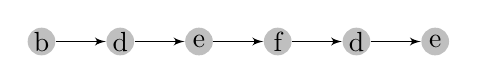
\begin{tikzpicture}[scale=1,auto,swap]
      \tikzset{edge/.style = {->,>=latex'}}
      \node[vertex] (a) at (0,0) {b};
      \node[vertex] (b) at (1,0) {d};
      \node[vertex] (c) at (2,0) {e};
      \node[vertex] (d) at (3,0) {f};
      \node[vertex] (e) at (4,0) {d};
      \node[vertex] (f) at (5,0) {e};
      \draw[edge] (a) to (b);
      \draw[edge] (b) to (c);
      \draw[edge] (c) to (d);
      \draw[edge] (d) to (e);
      \draw[edge] (e) to (f);
    \end{tikzpicture}

    \begin{itemize}
    \item {\bf Walk lengh:} 5 edges (The length of a walk is the EDGES, not the VERTICES)
    \item {\bf Representing as a compound relation:} $E(E(E(E(E(a)))))$
    \item NOTE: a walk can repeat edges and vertices! 
    \end{itemize}
  \end{block}

\end{frame}

\begin{frame}
  \frametitle{Path example}

  \begin{center}
    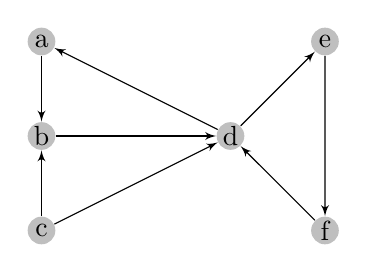
\begin{tikzpicture}[scale=1.2,auto,swap]
      \tikzset{edge/.style = {->,>=latex'}}
      \node[vertex] (a) at (0,1) {a};
      \node[vertex] (b) at (0,0) {b};
      \node[vertex] (c) at (0,-1) {c};
      \node[vertex] (d) at (2,0) {d};
      \node[vertex] (e) at (3,1) {e};
      \node[vertex] (f) at (3,-1) {f};
      \draw[edge] (a) to (b);
      \draw[edge] (c) to (b);
      \draw[edge] (b) to (d);
      \draw[edge] (d) to (a);
      \draw[edge] (c) to (d);
      \draw[edge] (d) to (e);
      \draw[edge] (e) to (f);
      \draw[edge] (f) to (d);
  \end{tikzpicture}
  \end{center}

  \begin{block}{Path: A walk without repeated vertices}

    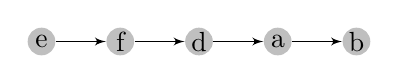
\begin{tikzpicture}[scale=1,auto,swap]
      \tikzset{edge/.style = {->,>=latex'}}
      \node[vertex] (a) at (0,0) {e};
      \node[vertex] (b) at (1,0) {f};
      \node[vertex] (c) at (2,0) {d};
      \node[vertex] (d) at (3,0) {a};
      \node[vertex] (e) at (4,0) {b};
      \draw[edge] (a) to (b);
      \draw[edge] (b) to (c);
      \draw[edge] (c) to (d);
      \draw[edge] (d) to (e);
    \end{tikzpicture}\hspace{1cm} {\bf Stuck!}

    \begin{itemize}
    \item {\bf Path lengh:} 4 edges (The length is counted in EDGES, not vertices)
    \item {\bf \structure{Eulerian Walk:}} Every \structure{edge} is visited once ({\bf E}ulerian).
    \item {\bf \alert{Hamiltonian Path:}} Every \alert{vertex} is visited once.
    \item {\bf Eulerian / Hamiltonian Circuit}: You go back to the initial vertex
    \end{itemize}
  \end{block}
\end{frame}

\begin{frame}{Proofs with Walks and Paths}
  \begin{proof}[Proof: The shortest Walk between two vertices is a Path]
    {\bf Proof by contradiction:} Assume a shortest walk that is not a path.

    \begin{enumerate}
    \item The shortest walk between $v_0$ and $v_n$ is not a path. So it has a repeated vertice $v_k$:
    \begin{equation*}
      w_{0,n} = v_0 \to v_1 \to \ldots \to v_k \to \ldots \to v_k \to \ldots \to v_{n-1} \to v_n
    \end{equation*}

    \item $w_{0,n}$  contains a smaller walk $w_{k,k}$ from $v_k$ to $v_k$ of size $|w_{k,k}| \geq 1$.
    \item We can remove $w_{k,k}$ from $w_{o,n}$, resulting in a smaller walk $w_{0,2}'$ with size $|w_{0,n}| - |w_{k,k}|$
    \item $w_{0,n}'$ is a walk from $v_0$ to $v_n$ that is shorter than $w_{0,n}$, which is a contradiction.
    \end{enumerate}
  \end{proof}

  This can be used to prove the \structure{Triangle Inequality} in walks (the distance of $i,j$ is equal or smaller than the distance from $i,k$ + $k,j$)

\end{frame}

\begin{frame}[t]{The Walk Relation}

  Let's describe a binary relation between vertices $v_i$ and $v_j$ in graph $G$,\\ and call it the \structure{Walk Relation}: 
  \begin{equation*}
    v_i G^n v_j.
  \end{equation*}

  The relation $G^n$ means: "There is a walk from $v_i$ to $v_j$ with length exactly $n$."\bigskip

  Let's think about $G^n$:
  \begin{itemize}
    \item $G^0$ is the set of all vertices (walk of size 0 goes nowhere)
    \item $G^1$ is the set of all pairs of vertices connected by 1 edge    
    \item {\bf composition and addition:} $G^n \circ G^m = G^{n+m}$ \hspace{.5cm}\\
    (For example, $G^2 + G^3 = G^5$)
    \item {\bf common vertex:} If there is a composite relation between $v_x$ and $v_y$ ($v_x~G^m \circ G^n~v_y$), this implies that there is a common vertex connecting them:\\
    $v_x~G^m \circ G^n~v_y\rightarrow \exists z, v_x~G^m~v_k, v_k~G^n~v_y$

  \end{itemize}
\end{frame}

\begin{frame}[t]{The Walk Relation and the Adjacency Matrix}

  Before, we described the Adjacency Matrix $A$, where $A_{i,j}=1$ if $E(v_i$,$v_j)$.
  \bigskip
  
  If we rename $A$ to $A_{G^1}$, we can generalize this concept to the \structure{Walk Matrix $A_{G^n}$}, which is the adjacency matrix representing $G^n$: $A_{G^n,i,j}=1$ if $v_i~G^n~v_j$. ($\exists$ walk of size $n$ from $v_i$ to $v_j$)
  \bigskip

  It is possible to calculate $A_{G^n}$ using \emph{boolean matrix multiplication}: $A_{G^n\circ G^m} = A'_{G^n} \odot A''_{G_m}$:

  \begin{equation*}
    a_{ij} = A'_{i*} \odot A''_{*j} = (a'_{i0} \land a''_{0j}) \lor (a'_{i1} \land a''_{1j}) \lor (a'_{i2} \land a''_{2j}) \lor \ldots \lor (a'_{in} \land a''_{nj})
  \end{equation*}\medskip

  This means that we can calculate $A_{G^n}$ quickly using the \structure{Fast Matrix Exponentiation}:

  \begin{itemize}
    \item $A_{G^n} = A_{G^{n/2}} \odot A_{G^{n/2}} = (A_{G^{n/4}} \odot A_{G^{n/4}}) \odot (A_{G^{n/4}} \odot A_{G^{n/4}}) = \ldots$
  \end{itemize}

\end{frame}

\begin{frame}[t]{Walk Relation $G^*$ of a Digraph}

  \begin{itemize}
  \item $G^n$ is the \structure{length $n$ walk relation}: It representes \structure{all walks of size exaclty $n$}
  \item $G^*$ is the \alert{walk relation of $G$}: It representes \alert{all walks in $G$}.
  \item $u G^* v$ means that \alert{there is a walk of {\bf some} length from $u$ to $v$}\\
  \end{itemize}\bigskip

  \structure{QUIZ:} How do we calculate $A_{G^*}$ for a graph, given adjacency matrix $A_{G^1}$?\bigskip

  \alert{HINT:} Remember that a walk can be infinite. But we need to solve this problem with a {\bf finite} algorithm! When does the algorithm stop?
\end{frame}

\begin{frame}[t]{Walk Relation of a DiGraph}{How to calculate $G^*$}

  \begin{enumerate}
  \item Let $G^1$ be the relation defined by the original graph (or its adjacency matrix).\medskip

  \item Let $G^0$ be the relation defined by the set $V$ with self:
    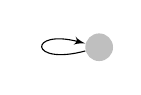
\begin{tikzpicture}[scale=1.5,auto,swap]
      \tikzset{edge/.style = {->,>=latex'}}
      \node[vertex] (a) at (0,0) {};
      \draw[edge] (a) to[loop left] (a);
    \end{tikzpicture}\\
    ($A_{G^0}$: the identity matrix).\medskip

  \item The relation $G^{\leq 1} = G^0 \cup G^1$ is the relation for walks of \emph{length 1 or less};\\
  ($A_{G^\leq 1} = A_{G^0} \times A_{G^1}$)\medskip

  \item $G^* = (G^{\leq})^{n-1}$: All walks of size $n-1$ or less.\hfill ({\bf Q: Why not n?})\medskip 
  
  \item Using fast exponentiation, you can calculate $G^*$ in $\log n$ matrix boolean multiplications
  \end{enumerate}
\end{frame}

\begin{frame}[t]{Adjacency Matrices and Neural Networks}{Why did we just study this?}
  We just studied an algorithm that can quickly calculate all the walks in a directed graph.\bigskip 

  If the graph is also {\bf acyclic}, and the edges have {\bf weights} in them, this algorithm can be easily generalized to \structure{calculate the total weight between any two vertices}.\bigskip 

  This can be used to quickly calculate the weight between the input neuron and the output neuron of a very large network!\bigskip

  \structure{This is one reason why Matrix Multiplications are important for Machine Learning.}

  \vfill 
  (caveat emptor: it gets more complicated with loops, non-linear activation functions, etc)
\end{frame}

\subsection{Prerequisite Course Graphs}

\begin{frame}{Walks and Prerequisite Course Graphs}
  \begin{columns}
    \column{0.4\textwidth}
      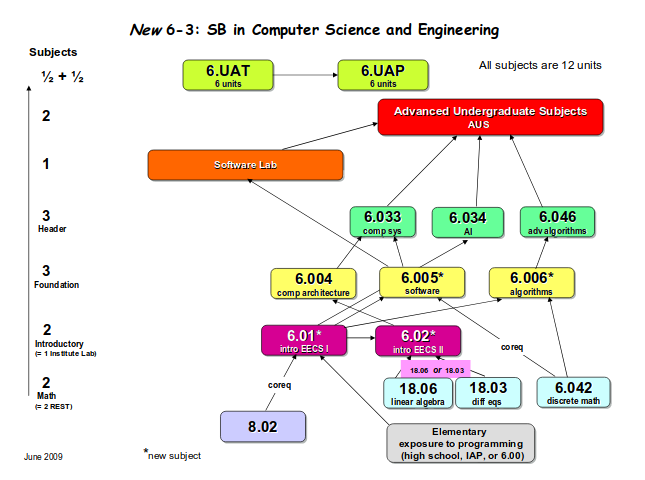
\includegraphics[width=1\textwidth]{../img/MIT_prereq}
      \pagenote{Course Pre-requisite image from "Math for CS" MIT OCW}
    \column{0.6\textwidth}
      The \emph{walk relation} of the pre-requisite graph $R$ defines how the courses relate to each other.
      \begin{itemize}
      \item \structure{Direct Prerequisite}: Req(6.046) = 6.006
      \item \structure{Indirect Prerequisite}: Req(6.046) = $\{6.006, 6.042, 6.01, 6.00, 8.02\}$
      \end{itemize}\medskip
  \end{columns}\bigskip

  Course $u$ is an indirect prerequisite of $v$ if there is a positive length walk from $u$ to $v$ in $R$:\medskip

  \begin{equation*}
    u D^+ v
  \end{equation*}
\end{frame}

\begin{frame}
  \frametitle{Requisites, Cycles and DAGs}

  In the beginning of the lecture, we talked about a prerequisite graph where it was not possible to graduate. Why? Because it had {\bf cycles}.\medskip

    \begin{itemize}
    \item A \structure{closed walk} is a walk that starts and ends at the same vertex.\medskip

    \item A \structure{cycle} is a closed walk where the only repeat
      vertex is at the beginning and end.
      \begin{itemize}
        \item $v_0 \to v_1 \to \ldots \to v_n \to v_0 | i > 0, j > 0, v_i \neq v_j$
        \item A cycle is the path $v \to w + (w,v)$
      \end{itemize}\medskip

    \item A \alert{Directed Acyclic Graph (DAG)} is a digraph that has
      \structure{no positive length cycles}.
    \end{itemize}
\end{frame}

\begin{frame}{Directed Acyclic Graphs Examples}

  Directed Acyclic Graphs (DAGs), can be used to represent several ordered structures:

    \begin{itemize}
      \item Course Prerequisite Graphs;
      \item Ordered Task List:
      \begin{itemize}
        \item "first add rice, then add water, then press cook button"
        \item "Let x be 5, let y be 2, while y $>$ 0, multiply x by x and subtract 1 from y."
      \end{itemize}
    \end{itemize}
    \bigskip

  Computational structures can also be described using DAGs:\medskip

    \begin{itemize}
      \item Relations, for example:
      \begin{itemize}
        \item \structure{Successor Relation}: $n \to n+1$
        \item \structure{Subset Relation}: $\{1,2\} \subset \{1,2,3\}$
      \end{itemize}
      \item Induction Proofs: ($P(n) \implies P(n+1) \implies P(n+2) \ldots$);
      \item Dynamic Programming: (base cases and transitions on the DP table);
    \end{itemize}
\end{frame}

\begin{frame}
  \frametitle{Directed Acyclic Graphs (DAG) and covering edges}

  \begin{columns}
    \column{0.3\textwidth}
    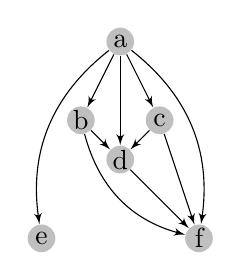
\begin{tikzpicture}[scale=.5,auto,swap]
      \tikzset{edge/.style = {->,>=latex'}}
      \node[vertex] (a) at (2,5) {a};
      \node[vertex] (b) at (1,3) {b};
      \node[vertex] (c) at (3,3) {c};
      \node[vertex] (d) at (2,2) {d};
      \node[vertex] (e) at (0,0) {e};
      \node[vertex] (f) at (4,0) {f};
      \draw[edge] (a) to (b);
      \draw[edge] (a) to (c);
      \draw[edge] (a) to (d);
      \draw[edge] (c) to (f);
      \draw[edge] (d) to (f);
      \draw[edge] (c) to (d);
      \draw[edge] (b) to (d);
      \draw[edge] (a) to[bend right] (e);
      \draw[edge] (a) to[bend left] (f);
      \draw[edge] (b) to[bend right] (f);
    \end{tikzpicture}

    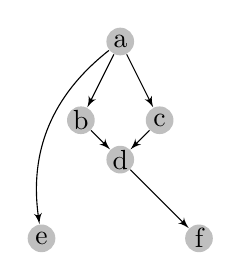
\begin{tikzpicture}[scale=.5,auto,swap]
      \tikzset{edge/.style = {->,>=latex'}}
      \node[vertex] (a) at (2,5) {a};
      \node[vertex] (b) at (1,3) {b};
      \node[vertex] (c) at (3,3) {c};
      \node[vertex] (d) at (2,2) {d};
      \node[vertex] (e) at (0,0) {e};
      \node[vertex] (f) at (4,0) {f};
      \draw[edge] (a) to (b);
      \draw[edge] (a) to (c);
      \draw[edge] (d) to (f);
      \draw[edge] (c) to (d);
      \draw[edge] (b) to (d);
      \draw[edge] (a) to[bend right] (e);
    \end{tikzpicture}

    \column{0.7\textwidth}

      Given a DAG $A$, its \structure{covering edges} is the {\bf smallest} DAG $B$ that has the same \structure{Walk Relation} as $A$\bigskip

      Walk relation of $A$ and $B$:
      \begin{itemize}
      \item $a\to \{b,c,d,e,f\}$
      \item $\{b,c\}\to \{d,f\}$
      \item $d\to f$
      \item $\{e,f\} \to \emptyset$
      \end{itemize}
  \end{columns}
\end{frame}

\section{Scheduling and Partial Orders}

\frame{
{Part 3: Scheduling and Partial Orders}

\tableofcontents[currentsection,hideallsubsections, firstsection=1, sections={1-4}]
}

\subsection{Scheduling}

\begin{frame}
  \frametitle{Using DAGs for Scheduling}

  Let's consider again using DAGs for calculating course prerequisites.\medskip

  \begin{columns}[T]
    \column{0.3\textwidth}
    $18.01 \rightarrow 6.042$\\
    $18.01 \rightarrow 18.02$\\
    $18.01 \rightarrow 18.03$
    \column{0.35\textwidth}
    $6.001 \rightarrow 6.034$\\
    $6.042 \rightarrow 6.046$\\
    $8.02 \rightarrow 6.002$\\
    $18.03, 6.002 \rightarrow 6.004$
    \column{0.35\textwidth}
    $6.001, 6.004 \rightarrow 6.033$\\
    $6.033 \rightarrow 6.857$\\
    $6.046 \rightarrow 6.840$
  \end{columns}

  \vfill

  We say that $u$ is a \structure{indirect prerequisite} of $v$ if there is a positive length walk in graph $R$:

    \begin{center}
      $18.01 \rightarrow 6.042 \rightarrow 6.046 \rightarrow 6.840$
    \end{center}
\end{frame}



\begin{frame}{DAGs and Scheduling}{Minimal, Minimum, Maximal, Maximum of a DAG}
  \begin{columns}
    \column{0.4\textwidth}
      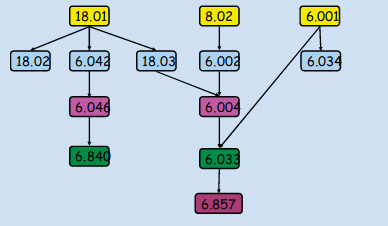
\includegraphics[width=1\textwidth]{../img/greedy_schedule}

      \column{0.6\textwidth}
    \begin{itemize}
    \item A \structure{minimal} course is does not have any prerequisites:
    \begin{itemize}
      \item $\emptyset \to 18.01$, $\emptyset \to 6.001$, $\emptyset \to  8.02$
    \end{itemize}\bigskip

    \item A \structure{minimum} course is an indirect prerequisite of {\bf all} courses.
    \begin{itemize}
      \item none in this example!
      \item if we add a course $x \to \{18.01, 8.02, 6.001\}$, then $x$ would be the minimum.
    \end{itemize}\bigskip

    \item \structure{Maximal} and \structure{maximum} courses have a similar definition.
    \begin{itemize}
      \item $\{18.02, 6.840, 6.857, 6.034\}\to \emptyset$ are maximal.
    \end{itemize}
    \end{itemize}
  \end{columns}
\end{frame}

\begin{frame}{DAG and Scheduling}{How to Schedule}

  \begin{columns}
    \column{0.4\textwidth}
      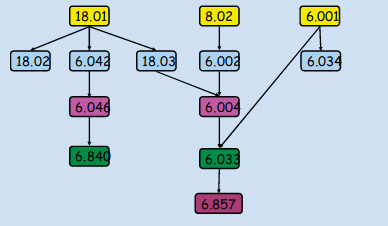
\includegraphics[width=1\textwidth]{../img/greedy_schedule}

    \column{0.6\textwidth}
      If we have the graph of course requirements, how do we select the courses for each semester? \medskip

      \structure{Greedy Scheduling}:
      \begin{enumerate}
      \item Identify Minimal Subjects;
      \item Add Minimal Subjects to Schedule;
      \item Remove Minimal Subjects;
      \item Return to Step 1
      \end{enumerate}
  \end{columns}\medskip

  Schedule:\\
  $\{18.01, 8.02, 6.001\} \to \{18.02, 6.042, 18.03, 6.002, 6.034\} \to \{6.046, 6.004\} \to \{ 6.840, 6.033\} \to 6.857$
\end{frame}


\begin{frame}{DAG and Scheduling}{Anti-Chains}
  \begin{columns}
  \column{0.4\textwidth}
    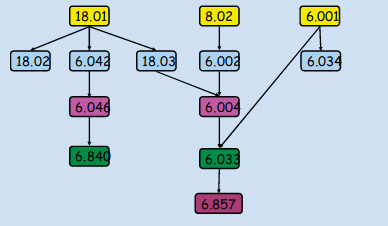
\includegraphics[width=1\textwidth]{../img/greedy_schedule}

  \column{0.6\textwidth}

    \begin{itemize}
    \item An \structure{anti-chain} is a set of vertices (courses) where there is no direct or indirect requisite relation among them.\medskip

    \item This means that the courses in an anti-chain can be taken in any order, even all at the same time.\medskip

    \item Members of an anti-chain are \structure{imcomparable}: It is not possible to say which one comes first.\medskip

    \item A relation graph can have multiple anti-chains. Example:
    \begin{itemize}
      \item $\{6.046, 6.004\}$
      \item $\{6.046, 18.03, 6.001\}$
    \end{itemize}
    \end{itemize}
  \end{columns}
\end{frame}

\begin{frame}{DAG and Scheduling}{Chains and Topological Sort}

  \begin{block}{Chains}
    Just like anti-chain is a set of vertices that have no relation among themselves, a \structure{chain} is a set of vertices that {\bf all} have a relation among themselves.
  \end{block}\medskip

  Using of chains and anti-chains, we define a \structure{Topological Sort}. A topological sort is an ordering of all vertices in $G$ that obeys the requisite relations.
  \begin{itemize}
    \item 18.01, 6.001, 8.02, 6.002, 18.03, 6.034, 6.042, 18.02, 6.004, 6.046, 6.033, 6.840, 6.857
    \item 6.001, 8.02, 6.002, 18.01, 6.034, 18.03, 18.02, 6.042, 6.004, 6.046, 6.033, 6.857, 6.840
  \end{itemize}
  If $G$ has anti-chains, it will also have multiple topological sorts.

\end{frame}

\begin{frame}{DAG and Scheduling}{Parallel Processing}

  We can use the same way of thinking to describe \structure{parallel scheduling} of tasks.\bigskip

  \begin{itemize}
    \item $n$ tasks have to be executed by $p$ processors.
    \item some pairs of tasks have a {\bf prerequisite} relation.
    \item \structure{Minimum Parallel Time}: minimum time to complete all tasks (assuming no limits on $p$)
      \begin{itemize}
        \item Minimum Parallel Time = Maximum Chain Size
      \end{itemize}
    \item \structure{Maximum Parallel Load}: value of $p$ necessary to achieve the Minimum Parallel Time
    \begin{itemize}
      \item Maximum Parallel Load $\leq$ Maximum Anti-chain Size
    \end{itemize}
  \end{itemize}
\end{frame}

\section{Partial Orders and Equivalence}

\begin{frame}{Partial orders: Transitivity}

  In a graph $G$, if there is a walk from $u$ to $v$, and a walk from $v$ to $w$, then there is a walk from $u$ to $w$
  \begin{center}
    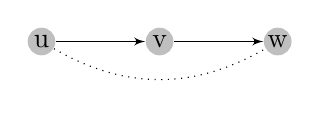
\begin{tikzpicture}[scale=.5,auto,swap]
      \tikzset{edge/.style = {->,>=latex'}}
      \node[vertex] (a) at (0,0) {u};
      \node[vertex] (b) at (3,0) {v};
      \node[vertex] (c) at (6,0) {w};
      \draw[edge] (a) to (b);
      \draw[edge] (b) to (c);
      \draw[dotted] (a) to[bend right] (c);
    \end{tikzpicture}
  \end{center}\bigskip

  Representing this in terms of \structure{walk relation} in $G$:
  \begin{equation*}
    uG^+v \land vG^+w \implies uG^+w
  \end{equation*}\bigskip

  \begin{block}{Definition: Transitive Relations}
    A relation {\bf R} is transitive if:\hspace{1cm} $xRy \land yRz \implies xRz$
  \end{block}
\end{frame}

\begin{frame}{Partial Orders: Assimetry}

  In an \structure{acyclic digraph G}, we can observe that for any two vertices $v$ and $u$, if there is a walk from $v$ to $u$, then there is no walk from $u$ to $v$.\bigskip

  \begin{block}{Definition: Assimetric Relation}
    A relation {\bf R} is assimetric if: $uD^+v \implies \text{NOT}(vD^+u)$
  \end{block}
\end{frame}

\begin{frame}{Strict Partial Order}

  A relation $R$ is a \structure{Strict Partial Order}(SPO) {\bf iff} it is {\bf Transitive} and {\bf Assimetric}.\bigskip

  Examples:
  \begin{itemize}
  \item The $\subset$ relation on sets
  \item The ``indirect prerequisite'' relationship on subjects.
  \item The $<$ relationship on $\mathbb{R}$
  \end{itemize}\bigskip

  Another way to say it, is that $R$ is a \structure{SPO} {\bf iff} $R$ is the walk relation $D^+$ for some DAG $D$.
\end{frame}

\begin{frame}{Path Total Orders}

    A \structure{Strict Partial Order} is also \structure{Path Total} if, for any two distinct elements, one will always be ``greater than'' another.

    \bigskip

    Example: $<$ on $\mathbb{R}$: if $x,y \in \mathbb{R},
    x\neq y \implies x>y \text{ or } y>x$

    \bigskip

    Counter-Example: $\subset$ in POW($\mathbb{N}$): $\{1,3\} \not\subset \{2,5\} \not\subset \{1,3\}$

    \vfill

    \begin{itemize}
    \item Relation $R$ is \structure{path total}: if $x \neq y \implies xRy \lor yRx$
    \item This means there are \alert{no imcomparable elements}
    \end{itemize}

    In a \structure{path total} relation, the whole graph is a
    \structure{chain}
  \begin{center}
    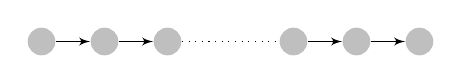
\begin{tikzpicture}[scale=.8,auto,swap]
      \tikzset{edge/.style = {->,>=latex'}}
      \node[vertex] (a) at (0,0) {};
      \node[vertex] (b) at (1,0) {};
      \node[vertex] (c) at (2,0) {};
      \node[vertex] (d) at (4,0) {};
      \node[vertex] (e) at (5,0) {};
      \node[vertex] (f) at (6,0) {};
      \draw[edge] (a) to (b);
      \draw[edge] (b) to (c);
      \draw[dotted] (c) to (d);
      \draw[edge] (d) to (e);
      \draw[edge] (e) to (f);
    \end{tikzpicture}
  \end{center}
\end{frame}

\begin{frame}{Weak Partial Order}

  A \structure{weak partial order} is the same as a \structure{strict
    partial order} R, except that $aRa$ always holds:
  \begin{center}
    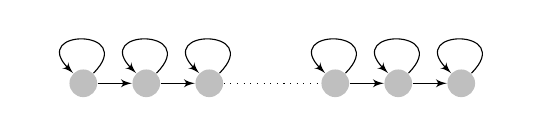
\begin{tikzpicture}[scale=.8,auto,swap]
      \tikzset{edge/.style = {->,>=latex'}}
      \node[vertex] (a) at (0,0) {};
      \node[vertex] (b) at (1,0) {};
      \node[vertex] (c) at (2,0) {};
      \node[vertex] (d) at (4,0) {};
      \node[vertex] (e) at (5,0) {};
      \node[vertex] (f) at (6,0) {};
      \draw[edge] (a) to (b);
      \draw[edge] (b) to (c);
      \draw[dotted] (c) to (d);
      \draw[edge] (d) to (e);
      \draw[edge] (e) to (f);
      \draw[edge] (a) to[loop] (a);
      \draw[edge] (b) to[loop] (b);
      \draw[edge] (c) to[loop] (c);
      \draw[edge] (d) to[loop] (d);
      \draw[edge] (e) to[loop] (e);
      \draw[edge] (f) to[loop] (f);
    \end{tikzpicture}
  \end{center}

  \bigskip

  \begin{itemize}
  \item Examples: $\subseteq$ on sets, $\leq$ on $\mathbb{R}$
  \item Weak Partial Orders define the property of
    \structure{Reflexivity}
  \item Relation $R$ on $A$ is \structure{reflexive} {\bf iff} $aRa,
    \forall a\in A$
  \end{itemize}

  Another way to define a weak partial order is that $R$ is a WPO {\bf iff}\\ $R = D^*$ for some DAG $D$
\end{frame}

\begin{frame}
  \frametitle{Assimetry and Antissimetry}

  {\larger

    \begin{block}{Assimetry}
      \begin{itemize}
      \item Reflexibility is \alert{never} allowed
      \item R is \structure{assimetric} {\bf iff}:
        \begin{equation*}
          xRy \implies \text{NOT}(yRx)
        \end{equation*}
      \end{itemize}

    \end{block}

    \begin{block}{Antissimetry}
      \begin{itemize}
      \item Reflexibility is \alert{sometimes} allowed
      \item R is \structure{antissimetric} {\bf iff}
        \begin{equation*}
          xRy \implies \text{NOT}(yRx), \text{ for } x \neq y
        \end{equation*}
      \end{itemize}
    \end{block}
  }
\end{frame}


\subsection{Partial Orders and Isomorphisms}

\begin{frame}{Partial Orders and Isomorphism}{Proper Subset Relation}
  \frametitle{Proper Subset Relation}

  The proper subset relation: $A \subset B$ represents a partial order.\bigskip

  For example, the proper subset relation defined on the power set of $\{1,2,3,5,10,15,30\} - \emptyset$ is as follows:

\begin{center}
    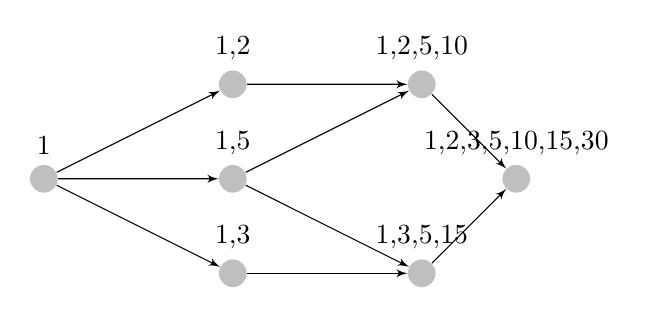
\begin{tikzpicture}[scale=1.2,auto,swap]
      \tikzset{edge/.style = {->,>=latex'}}
      \node[vertex,label={1}] (a) at (0,1) {};
      \node[vertex,label={1,3}] (b) at (2,0) {};
      \node[vertex,label={1,5}] (c) at (2,1) {};
      \node[vertex,label={1,2}] (d) at (2,2) {};
      \node[vertex,label={1,3,5,15}] (e) at (4,0) {};
      \node[vertex,label={1,2,5,10}] (f) at (4,2) {};
      \node[vertex,label={1,2,3,5,10,15,30}] (g) at (5,1) {};
      \draw[edge] (a) to (b);
      \draw[edge] (a) to (c);
      \draw[edge] (a) to (d);
      \draw[edge] (c) to (e);
      \draw[edge] (b) to (e);
      \draw[edge] (c) to (f);
      \draw[edge] (d) to (f);
      \draw[edge] (e) to (g);
      \draw[edge] (f) to (g);
    \end{tikzpicture}
  \end{center}
\end{frame}

\begin{frame}{Partial Orders and Isomorphism}{Proper Divide Relation}

  The \structure{proper divide} relation is defined as $a R b$ if $a|b$ and $a \neq b$.\bigskip

  We can see that, for the set $\{1,2,3,5,10,15,30\}$, the proper subset relation and the proper division relation have {\bf the same relationship DAG}.\bigskip

  This means that the two relations are \structure{{\bf isomorphic}}

  \begin{center}
    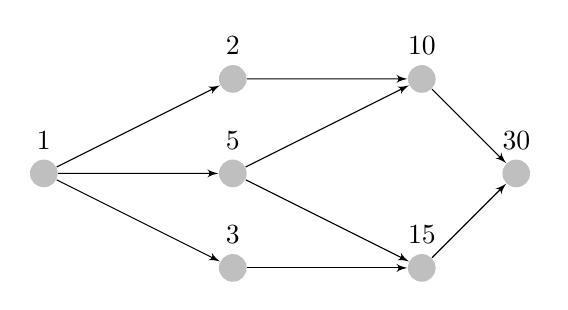
\begin{tikzpicture}[scale=1.2,auto,swap]
      \tikzset{edge/.style = {->,>=latex'}}
      \node[vertex,label={1}] (a) at (0,1) {};
      \node[vertex,label={3}] (b) at (2,0) {};
      \node[vertex,label={5}] (c) at (2,1) {};
      \node[vertex,label={2}] (d) at (2,2) {};
      \node[vertex,label={15}] (e) at (4,0) {};
      \node[vertex,label={10}] (f) at (4,2) {};
      \node[vertex,label={30}] (g) at (5,1) {};
      \draw[edge] (a) to (b);
      \draw[edge] (a) to (c);
      \draw[edge] (a) to (d);
      \draw[edge] (c) to (e);
      \draw[edge] (b) to (e);
      \draw[edge] (c) to (f);
      \draw[edge] (d) to (f);
      \draw[edge] (e) to (g);
      \draw[edge] (f) to (g);
    \end{tikzpicture}
  \end{center}
\end{frame}

\begin{frame}{Isomorphism}

    \begin{itemize}
    \item Two graphs are \structure{isomorphic} if they have the same \structure{set of vertices and set of edges}\bigskip

    \item More formally, two graphs $G_1, G_2$ are \structure{isomorphic} if there is a relation $M$ which is an \emph{edge preserving maching} between their vertices.\bigskip

    \item $G_1 \text{ isomorphic } G_2 \iff \exists \text { bijection
    } M:V_1\to V_2$\\\hfill with $(u,v) \in E_1 \iff
      (M(u),M(v)) \in E_2$

    \end{itemize}
\end{frame}

%% TODO: Remember why this is important and then re-add to the lecture
% \begin{frame}
%   \frametitle{Isomorphism, $\subset$ and partial orders}
%
%   {\larger
%     {\bf Theorem:} Every strict p.o. $R$ is isomorphic to some
%     collection of sets partially ordered by $\subset$.
%
%     \bigskip
%
%     {\bf Proof (by construction):}
%     \begin{itemize}
%     \item Map element $a$ to the set of elements below it.
%     \item in other words, $a$ maps to $\{b \in A| bRa \lor b = a\}$\\
%       \hfill(remember that NOT$(aRa)$)
%     \item in other words, $f(a) ::= R^{-1}(a) \cup \{a\}$
%     \end{itemize}
%
%     \bigskip
%
%     {\bf Example:} from divides
%     \begin{itemize}
%     \item $f(10) = 1|10, 2|10, 5|10, \cup \{10\} = \{1,2,5,10\}$
%     \item $f(3) = 1|3, \cup \{3\} = \{1,3\}$
%     \end{itemize}
%   }
% \end{frame}

\subsection{Equivalence Relations}

\begin{frame}
  \frametitle{Symmetric Relations and Equivalence Relations}

  \begin{itemize}
    \item If there is a walk from $u$ to $v$ and a walk from $v$ to
      $u$, then we say that $u$ and $v$ are \structure{strongly
      connected}.
      \begin{itemize}
        \item $uG^*v$ and $vG^*u$
      \end{itemize}\bigskip

    \item The relation $R$ is \structure{symmetric} if $aRb \implies bRa$.
    \begin{itemize}
      \item The walk relation of A \structure{strongly connected} graph is symmetric.
    \end{itemize}\bigskip

    \item An \structure{equivalence relation} $R$ is: transitive,
      symmetric and reflexive.\bigskip

    \item This means that $R$ is an \structure{equivalence relation} {\bf iff} $R$ is the \structure{strongly connected} relation of some DiGraph.
    \end{itemize}
\end{frame}

\begin{frame}
  \frametitle{Equivalence Relations Examples}

  The definitions of the last slide allows us to formally define an \emph{equivalence equation}.\bigskip

  {\larger
    Examples:
    \begin{itemize}
    \item Equality: $=$
    \item $\equiv $(mod n)
    \item Same Size, Same Color, etc.
    \end{itemize}
  }\bigskip

  It may seem that an equivalence relation is too obvious to need a definition (specially for numbers!), but this can be useful when we want to define equivalence for more complex things, like sets.

\end{frame}

\begin{frame}
  \frametitle{Relation Properties: Graphical Review}

  {\larger

    \begin{columns}
      \column{0.5\textwidth}
      \begin{center}
      Reflexive:\\
      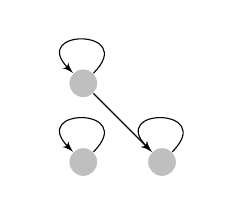
\begin{tikzpicture}[scale=1,auto,swap]
        \tikzset{edge/.style = {->,>=latex'}}
        \node[vertex] (a) at (0,0) {};
        \node[vertex] (b) at (1,0) {};
        \node[vertex] (c) at (0,1) {};
        \draw[edge] (a) to[loop] (a);
        \draw[edge] (b) to[loop](b);
        \draw[edge] (c) to[loop] (c);
        \draw[edge] (c) to (b);
      \end{tikzpicture}

      \bigskip

      Transitive:\\
      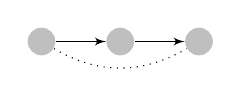
\begin{tikzpicture}[scale=1,auto,swap]
        \tikzset{edge/.style = {->,>=latex'}}
        \node[vertex] (a) at (0,0) {};
        \node[vertex] (b) at (1,0) {};
        \node[vertex] (c) at (2,0) {};
        \draw[edge] (a) to (b);
        \draw[edge] (b) to (c);
        \draw[dotted] (a) to[bend right] (c);
      \end{tikzpicture}
      \end{center}
      \column{0.5\textwidth}
      \begin{center}
      Assymetric:\\
      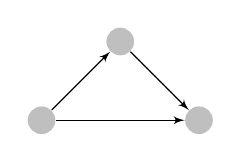
\begin{tikzpicture}[scale=1,auto,swap]
        \tikzset{edge/.style = {->,>=latex'}}
        \node[vertex] (a) at (0,0) {};
        \node[vertex] (b) at (1,1) {};
        \node[vertex] (c) at (2,0) {};
        \draw[edge] (a) to (b);
        \draw[edge] (b) to (c);
        \draw[edge] (a) to (c);
      \end{tikzpicture}

      \bigskip

      Symetric:\\
      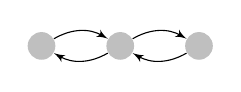
\begin{tikzpicture}[scale=1,auto,swap]
        \tikzset{edge/.style = {->,>=latex'}}
        \node[vertex] (a) at (0,0) {};
        \node[vertex] (b) at (1,0) {};
        \node[vertex] (c) at (2,0) {};
        \draw[edge] (a) to[bend left] (b);
        \draw[edge] (b) to[bend left] (a);
        \draw[edge] (b) to[bend left] (c);
        \draw[edge] (c) to[bend left] (b);
      \end{tikzpicture}

      \end{center}
    \end{columns}
  }
\end{frame}


% TODO: Remember why this is important and re-introduce it!
% \begin{frame}
%   \frametitle{Representing Equivalence}
%   {\larger
%
%     \begin{itemize}
%     \item For a total function $f:A\rightarrow B$
%     \item We can define an equivalence relation: $\equiv_f$ on $A$:
%       \begin{equation}
%         a \equiv_f a' \iff f(a) = f(a')
%       \end{equation}
%
%       \bigskip
%
%     \item {\bf Theorem:} Relation $R$ on set $A$ is an equiv. relation
%       {\bf iff}: $R$ is $\equiv_f$ for some $f:A\rightarrow B$
%
%       \bigskip
%
%     \item {\bf Example:} $\equiv$ (mod n) is $\equiv_f$
%       \structure{where} $f(k) ::= \text{rem}(k,n)$
%     \end{itemize}
%   }
% \end{frame}
%
% \begin{frame}
%   \frametitle{Equivalence and Partition}
%
%   {\larger
%     \begin{itemize}
%     \item We define a \structure{partition} $\Pi$ of a set $A$, where
%       $\$Pi$ is a collection of subsets of $A$ that cover all elements
%       but do not overlap.
%
%       \bigskip
%
%       {\bf Example:} For A = $\{a,b,c,d,e\}$ one partition could be:
%       $\{a,b\},\{c,e\},\{d\}$
%
%
%       \bigskip
%
%     \item We define a relatin $\equiv_{\Pi}$ on A: $a \equiv_{\Pi} a'$
%       if both $a$ and $a'$ are in the same subset of $\Pi$
%
%       \bigskip
%
%     \item A relation $R$ on set $A$ is an equivalence relation {\bf
%       iff} $R$ is $\equiv_{\Pi}$ for some partition $\Pi$ of $A$.
%     \end{itemize}
%
%   }
% \end{frame}

%%%%%%%%%%%%%%%%%%%%%%%%%%%%%%%%%%%

\section{Back Matter}
\begin{frame}{Slide Credits}
  These slides were made by Claus Aranha, 2020. You are welcome to copy, re-use and modify this material, following the CC-SA-NC license.
  \bigskip

  These slides are based on "Mathematics For Computer Science (Spring 2015)", by Albert Meyer and Adam Chlipala, MIT OpenCourseWare. \url{https://ocw.mit.edu}.
  \bigskip

  Individual images in some slides might have been made by other
  authors. Please see the following slides for information about these cases.
\end{frame}

\begin{frame}[allowframebreaks]{Image Credits}
  \printnotes
\end{frame}


\end{document}
